\documentclass[conference]{IEEEtran}
\IEEEoverridecommandlockouts
% The preceding line is only needed to identify funding in the first footnote. If that is unneeded, please comment it out.
%\usepackage{cite}
\usepackage[utf8]{inputenc}
\usepackage{amsmath,amssymb,amsfonts}
\usepackage{algorithmic}
\usepackage{graphicx}
\usepackage{textcomp}
\usepackage{xcolor}
\usepackage{multirow}
\usepackage{float}
\usepackage{subcaption}
\usepackage[backend=bibtex,sorting=none,style=ieee]{biblatex}
\addbibresource{paper.bib}
%\def\BibTeX{{\rm B\kern-.05em{\sc i\kern-.025em b}\kern-.08em
 %   T\kern-.1667em\lower.7ex\hbox{E}\kern-.125emX}}
\begin{document}

\title{Self-driving	through a deep recurrent convolutional neural model.}
\author{
	
\IEEEauthorblockN{Luna-Álvarez Antonio}
\IEEEauthorblockA{\textit{Depto. de Ciencias Computacionales.} \\
	\textit{CENIDET-TecNM}\\
	Cuernavaca, Mexico \\
	jesus.luna18ce@cenidet.edu.mx}

\and

\IEEEauthorblockN{Mújica-Vargas Dante}
\IEEEauthorblockA{\textit{Depto. de Ciencias Computacionales.} \\
	\textit{CENIDET-TecNM}\\
	Cuernavaca, Mexico \\
	dantemv@cenidet.edu.mx}

}
\maketitle

\begin{abstract}
The autonomous driving in cars is a task of great complexity due to the multiple factors to be considered. With the popularization of deep learning, great advances have been made in this domain, achieving acceptable results. However, a constant defect in the works reported in the literature is the lack of consideration of time as a factor of great importance, considering only current scenes being a reactive method. This document shows the experimentation with a recurrent convolutional neuronal model, which contemplates previous actions to take the current decisions.
\end{abstract}

\begin{IEEEkeywords}
Deep Learning, Convolutional Model, Recurrent Model, Time-distributed, Self-driving, Autonomy.
\end{IEEEkeywords}

\section{Introduction}
Autonomous vehicles are robotic systems that must have the ability to navigate through the environment for which they were designed, independently and avoiding obstacles or situations that compromise the safety of the vehicle and its passengers. The main component of a self-driving car is the decision module, which can be controlled by a classification model that will mainly predict the steering angle and vehicle speed \cite{litman2017autonomous}. In the study of the state of the art it has been observed that of the most reliable classification models are given by a Neural Network Based on Deep Learning (DNN).

Although good self-driving results have been documented using deep learning, the importance of time in the driving task has been ignored. A person with sufficient experience driving in urban areas foresees the following actions in advance, for example braking distances. In the same way it makes decisions taking into account the actions taken in previous immediate times. For example, the speed and angle of the vehicle after taking a curve, as shown in Fig. \ref{fig:comparsion}.

\begin{figure}[h]
	\centering
	\begin{subfigure}{0.22\textwidth} 
		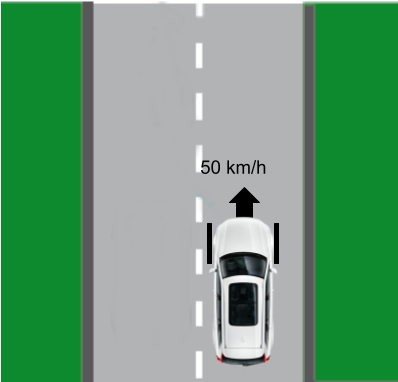
\includegraphics[width=\textwidth]{img/reactive}
		\subcaption{Scene that sees a reactive model.} 
		\label{subfig:reactive}
	\end{subfigure}
	\begin{subfigure}{0.22\textwidth} 
		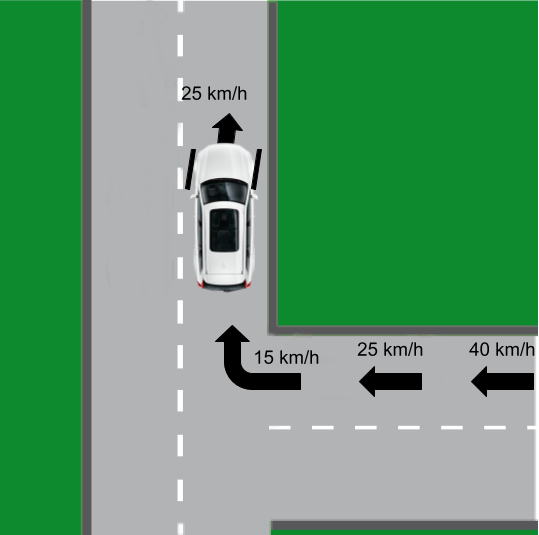
\includegraphics[width=\textwidth]{img/recurrent}
		\subcaption{Scene that sees a model based on time.} 
		\label{subfig:recurrent}
	\end{subfigure}
	\caption{Difference between reactive and time-based models.} 
	\label{fig:comparsion}
\end{figure}

Similar to how a human driver does it, a neural model dedicated to self-driving receives the image of the road as input. To interpret this image a Convolutional Neural Network (CNN) is used. This type of neural network extracts the most important characteristics, as could be the lines of the road. The information is processed by layers of classification in the architecture of the network, learning these characteristics and the commands (steering, acceleration or others) as a class. In practice, the network associates the input images with which it was trained and returns the command, as seen in Fig. \ref{subfig:reactive}.

However, this doesn't store the predictions of previous steps, which are necessary to make appropriate decisions to the situation. As shown in Fig. \ref{subfig:recurrent}, although the car is currently on a straight road, because I make a turn the speed is lower and it's necessary to correct the angle of the wheels.

The objective of this document is to show the recurrent convolutional neuronal paradigm and its performance in comparison with a reactive convolutional neuronal paradigm shown in the literature, in the task of self-driving.


\section{Background}

\subsection{Convolutional Neural Network}

The convolutional neural networks (CNN) are based on the convolution of signals in two dimensions and the detection of filter-based characteristics (called kernel) that they learn through training. To extract the characteristics, the kernel performs the 2D convolution operation, expressed in \eqref{eq:convolution}, to the input image. 

\begin{equation}
\begin{split}
y(n_1, n_2) = \sum_{k_2=0}^{N-1} \sum_{k_1=0}^{M-1} x(k_1, k_2)\ h(n_1 - k_1, n_2 - k_2)\\
0 \leq n_1 \leq N-1,\ 0 \leq n_2 \leq M - 1
\end{split}
\label{eq:convolution}
\end{equation}

Where $N$ and $M$ are the dimensions of the image, $n_1$ and $n_2$ represent the column and row indices of the pixel being processed, $k_1$ and $k_2$ the kernel indexes.\\

This type of neural network has great advantages of automation in the task of extracting image information. In this paradigm, no known image processing filter is applied, but through the training of the neural network, it learns the image processing filters. In general, the first convolution layer learns to detect edges, while the second can learn to detect more complex shapes that can be formed by combining different edges, such as circles and rectangles. The third layer and beyond learn much more complicated characteristics based on the characteristics generated in the previous layer \cite{pattanayak2017pro}.\\


To train the convolutional layers, the backpropagation through the convolutional layer technique is used. This is very similar to backpropagation for a multilayer perceptron network, the only difference being that the weight connections are scattered, since the different input areas share the same weights to create a map of output characteristics. In general, the map of characteristics is obtained through the function expressed in \eqref{eq:error}. Where w represents the weights of the kernel and a first map of characteristics obtained.

\begin{equation}
S_{ij} = \sum_{n=1}^{2} \sum_{m=1}^{2} w_{(3-m)(3-n)} \cdot a_{(i-1+m)(j-1+m)}
\label{eq:error}
\end{equation}

For convolutional layers, the assigned activation function is the Rectified Linear Unit Function (ReLU) which is expressed in \eqref{eq:relu} where $x$ represents the input value. This function allows normalizing the data by not admitting negative values and thus avoid noise that may contain the input image.

\begin{equation}
ReLU = ln(1+e^x)
\label{eq:relu}
\end{equation}

On the other hand, the kernel weights are adjusted by calculating the descending gradient which is expressed in \eqref{eq:gradient}. Where L represents the error function.
\begin{equation}
\frac{\partial L}{\partial w_{ij}} = \sum_{i=1}^{2} \sum_{j=1}^{2} \frac{\partial L}{S_{ij}} \frac{\partial S_{ij}}{\partial w_{ij}}
\label{eq:gradient}
\end{equation}


\subsection{Recurrent Neural Network}

Recurrent Neural Networks (RNN) are designed to use and learn from sequential information. Generally, an RNN can be viewed as a weighted, directed, and cyclic graph that contains three different types of nodes, which are; the input, hidden and output nodes \cite{zhang2016architectural}.\\

There are three types of essential tasks that can be performed with this type of network \cite{bonet2007redes}:

\begin{enumerate}
	\item Sequence recognition: A particular output pattern occurs when an input sequence is specified.
	
	\item Sequence playback: The network must be able to generate the rest of a sequence when you see part of it.
	
	\item Temporal association: In this case a particular output sequence must be produced in response to a specific input sequence.\\
\end{enumerate}

The RNN suffer from an inherent problem: they don't capture the long distance dependencies between the inputs. This is because gradients in instances of long sequences have a high probability of going quickly to zero, called vanishing of the gradient, or tending to infinity called explosion of the gradient.
A simple solution to the gradient explosion problem is to add a threshold that limits exponential growth. However, it isn't enough for the problem of gradient fading, so some variants of the classic RNN model have been proposed.\\

The Long Long-term Memory (LSTM) architecture was originally proposed by Hochreiter and Schmidhuber in 1997 \cite{hochreiter1997long}, and is widely used today due to its superior performance in accurate modeling of short and long term dependencies.

An LSTM neuron is composed of 5 different non-linear components, which interact with each other in a particular way. In this paradigm, 4 components are called gates, they protect and control the information in the cell, which stores the memory of the neuron. The gates are implemented by a sigmoid function and a inner product. To control the behavior of each gate, one trains with a set of parameters and by calculating the gradient descending. The 5 gates of an LSTM cell are expressed in \eqref{eq:rnn}.

\begin{subequations}
	\begin{equation}
	Forget\ gate: \sigma_f[t] = \sigma(\textbf{W}_f x[t]+\textbf{R}_f y[t-1]+b_f) 
	\end{equation}    
	\begin{equation}
	Candidate\ state: \tilde{\textbf{h}}_f[t] = g_1(\textbf{W}_h x[t]+\textbf{R}_h y[t-1]+b_h)
	\end{equation}
	\begin{equation}
	Update\ gate: \sigma_u[t] = \sigma(\textbf{W}_u x[t]+\textbf{R}_u y[t-1]+b_u)
	\end{equation}
	\begin{equation}
	Cell\ state: \textbf{h}[t] = \sigma_u[t] \odot \tilde{\textbf{h}}[t]+\sigma_f[t]\odot \textbf{h}[h-1]
	\end{equation}
	\begin{equation}
	Output\ gate: \sigma_o[t] = \sigma(\textbf{W}_o\textbf{x}[t]+\textbf{R}_o y[t-1]+\textbf{b}_o)
	\end{equation}
	\begin{equation}
	Output: \textbf{y}[t] = \sigma_o[t]\odot g_2(\textbf{h}[t])
	\end{equation}
	\label{eq:rnn}
\end{subequations}

Where $x[t]$ is the input vector at time $t$. $W_f$, $W_h$, $W_u$ and $W_o$ are rectangular weight matrices that are applied to the input of the LSTM cell. $R_f$, $R_h$, $R_u$ and $R_o$ are square matrices that define the weights of the recurrent connections, while $b_f$, $b_h$, $b_u$ and $b_o$ are vectors of bias. The function $\sigma(\cdot)$ is sigmoid, while $g_1(\cdot)$ and $g_2(\cdot)$ are point nonlinear activation functions generally implemented as hyperbolic tangents that reduce the values in $[-1, 1]$. Finally, $\odot$ represents the inner product \cite{bianchi2017recurrent}. 


\section{System description}

\subsection{Simulation \& Data}
The platform used to experiment with this approach is the Udacity simulator. This simulator presents a great advantage by providing a training module, which consists of a manual driving in which it can be recorded through three simulated cameras located in the front of the vehicle, each image has a size of 320 x 160 pixels and 3 color channels. The images obtained from the simulator can be seen in Fig. \ref{fig:cameras}, these three images represent a pattern of the driving database. The simulator captures 10 patterns per second, considering that the maximum speed of the vehicle is $30\ mi/h$, approximately each instance has a difference of 1 meter.


\begin{figure}[h]
	\centering
	\begin{subfigure}{0.22\textwidth} 
		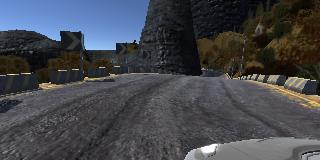
\includegraphics[width=\textwidth]{img/left}
		\caption{Left camera.} 
	\end{subfigure}
	\begin{subfigure}{0.22\textwidth} 
		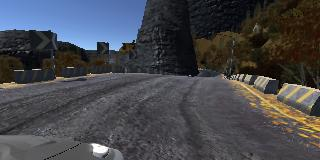
\includegraphics[width=\textwidth]{img/right}
		\caption{Right camera.} 
	\end{subfigure}
	\begin{subfigure}{0.22\textwidth} 
		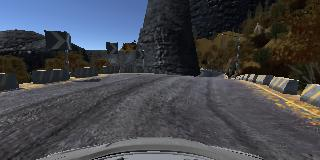
\includegraphics[width=\textwidth]{img/center}
		\caption{Center camera.} 
	\end{subfigure}
	\caption{Images obtained from manual driving in the Udacity simulator.} 
	\label{fig:cameras}
\end{figure}

The Udacity simulator provides a file in CSV format which contains the absolute path where that images are stored, as well as a vehicle steering command expressed in radians in a closed range $[-0.43, 0.43]$ (in the simulator is seen as $[-25^\circ, 25^\circ]$) which take the role of the class. Considering only 2 floating points, there's a difference between classes of $0.01\ r \Rightarrow 0.5729^\circ$, obtaining a total of 87 classes and avoiding a drastic turn of the vehicle.

The manual driving is done through the control with the keyboard for the actions of turning, accelerating and braking. However the keyboard doesn't have the sensitivity to make slight turns, it's necessary to press the key several times in short periods to maintain the correct direction. These actions become noise in the class as shown in Fig. \ref{subfig:key}. To solve this problem, a videogame steering wheel was used. Fig. \ref{subfig:joy} shows the steering commands obtained in the same fragment of the road driven with the steering wheel.

\begin{figure}[h]
	\centering
	\begin{subfigure}{0.4\textwidth} 
		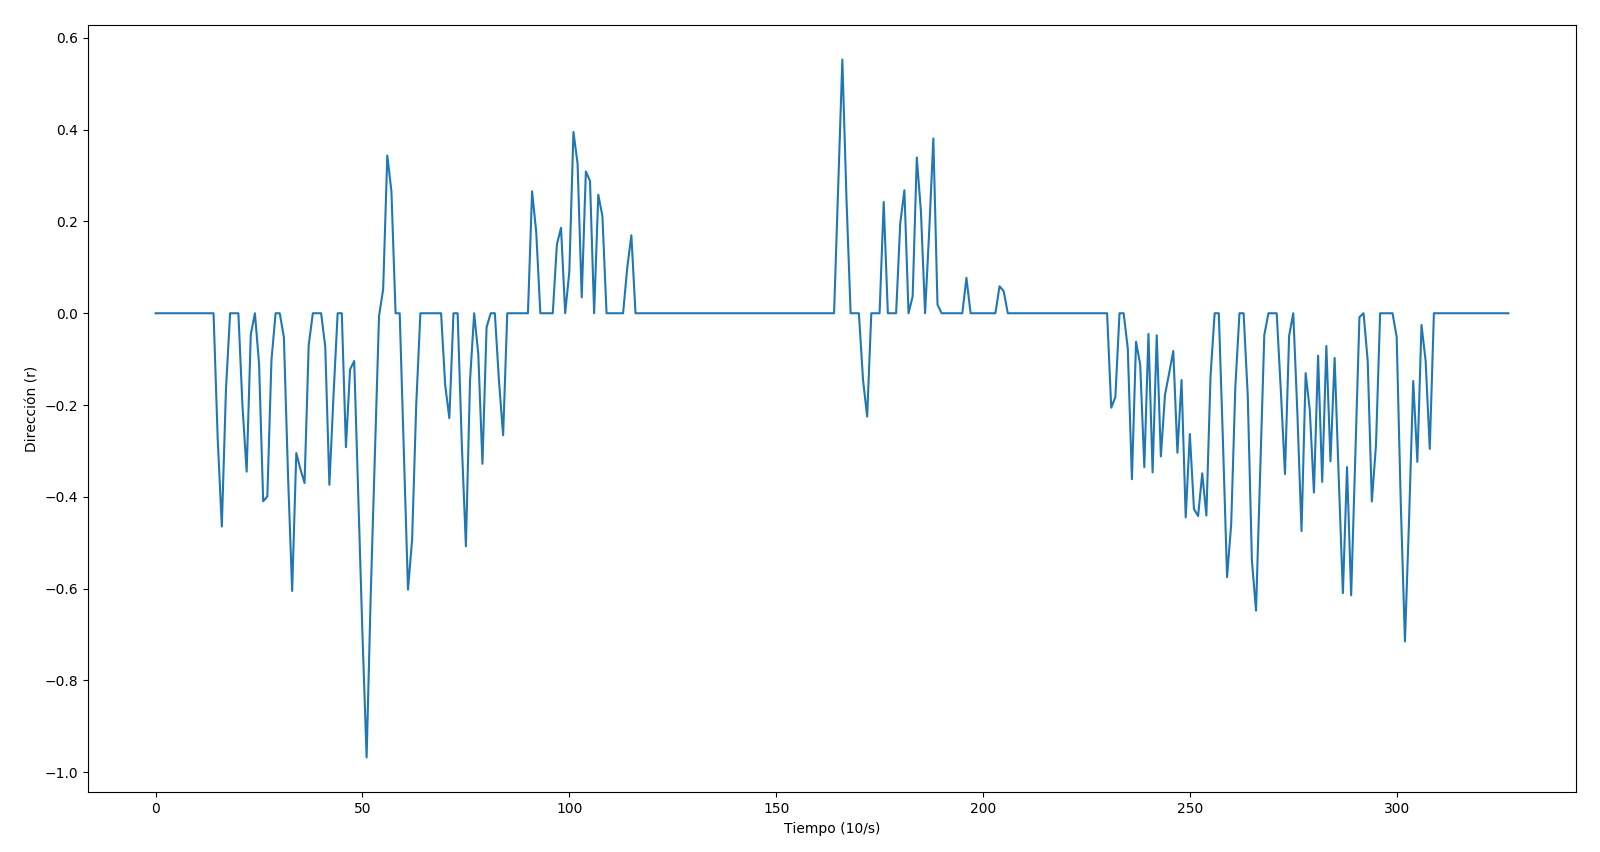
\includegraphics[width=\textwidth]{img/keyboard}
		\subcaption{Steering commands with keyboard.} 
		\label{subfig:key}
	\end{subfigure}
	\begin{subfigure}{0.4\textwidth} 
		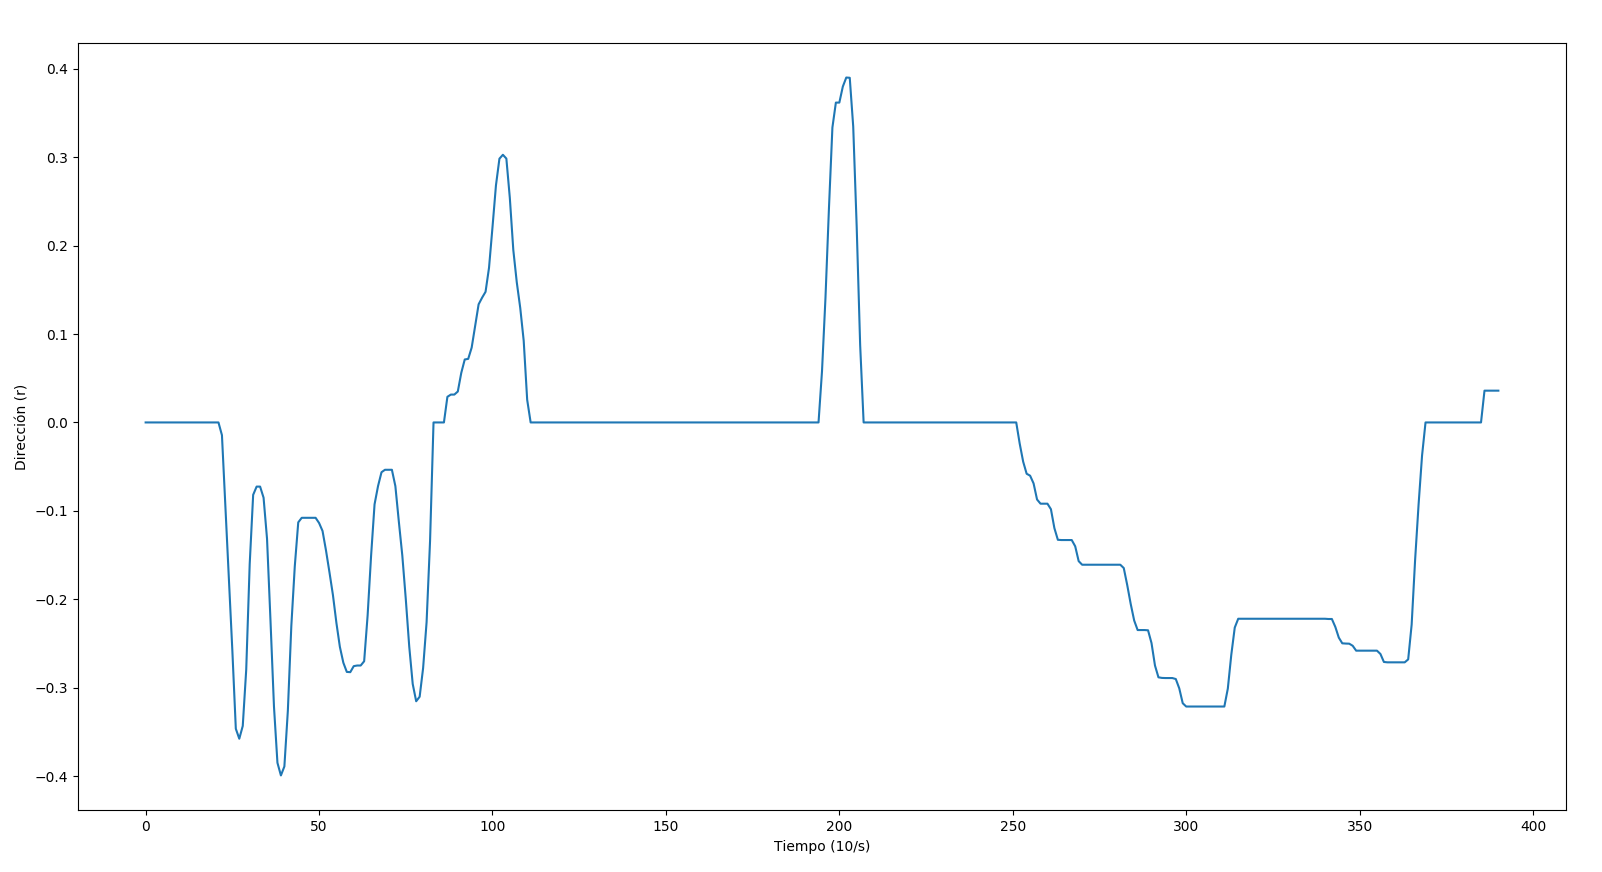
\includegraphics[width=\textwidth]{img/joystick}
		\subcaption{Steering commands with joystick.} 
		\label{subfig:joy}
	\end{subfigure}
	\caption{Vehicle steering commands (class).} 
\end{figure}

Now with respect to the evaluation of driving and because the developers of Udacity don't provide data on the length of the tracks, manual driving was performed at a constant speed of $30 mi/h$ (maximum speed), measuring the time to complete the The longitude result for the first track of $1.28\ km$ ($0.8\ mi$) and $2.99\ km$ ($1.86\ mi$) for the second was reached. This information is very important to evaluate the performance of models trained in the task of driving.

\subsection{Preprocesing}

The simulator only has two tracks: a simple one of approximately 2 miles and the other more complicated of double length. Therefore, if a model trained in these scenarios was tested in another environment with different lighting and road conditions, the network wouldn't give the expected results. Therefore, a preprocessing is carried out in two stages:

\begin{enumerate}
	\item A clipping is made in the input image (which is 320 x 160 pixels) by removing 25 pixels in the lower part and 60 in the upper one, thus eliminating the front part of the vehicle that appears in the image and the sky that doesn't provide useful information, as shown in Fig. \ref{fig:cutted}. 
	
	The image is also scaled to a new one of 200 x 66 pixels, this to make the processing in the convolutional layers a little lighter and thus obtain a data vector of smaller size.
	
	\begin{figure}[H]
		\centerline{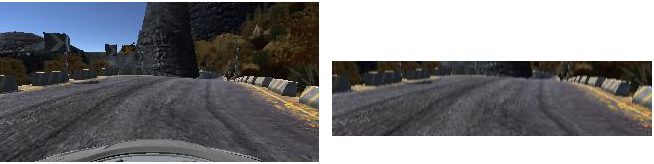
\includegraphics[scale=0.36]{img/cutted}}
		\caption{Image clipping.}
		\label{fig:cutted}
	\end{figure}
	
	\item In this stage, the selection of one of the views shown in Fig. \ref{fig:cameras} is made. This serves as an information increase, since if the manual driving is carried out ideally maintaining a good position in the lane, cases in which the vehicle is near the edge of the road or invading the opposite lane wouldn't be memorized by the network and wouldn't respond adequately before this situation. Therefore a selection of one of the three views and their respective direction adjustment, expressed in \eqref{eq:views}, represents three different patterns.
	
	\begin{equation}
		f(r) =
		\begin{cases}
		r+0.2       & \quad \text{if } view = 0\\
		r-0.2  & \quad \text{if } view = 1\\
		r & \quad other
		\end{cases}
		\label{eq:views}
	\end{equation}
	
	In addition, a random rotation is performed on the $X$ axis by adjusting the direction command given a random value $x$, $r = r + (x * 0.002)$. This visually represents a more closed or open curve as the case may be.
	
	There may also be a rotation of the image generating a scene contrary to the existing one. The direction command is adjusted given $r = r * -1.0$, totally inverting the direction, as well as the original image.
\end{enumerate}



\subsection{Recurrent Convolutional Model}
Because the design of an architecture requires extensive experimentation and extensive knowledge of the subject, the model proposed by \cite{tian2018deeptest} was used, which is used to decide turning angles in static images of roads with extreme climatic conditions. This model shown in Fig. \ref{fig:chauffeur} is made up of 5 convolutional layers, it doesn't have pooling layers. For the classification, 3 LSTM layers are used and finally 2 Multilayer Perceptron, the last one with a neuron to give the command as an output.

\begin{figure}[h]
	\centerline{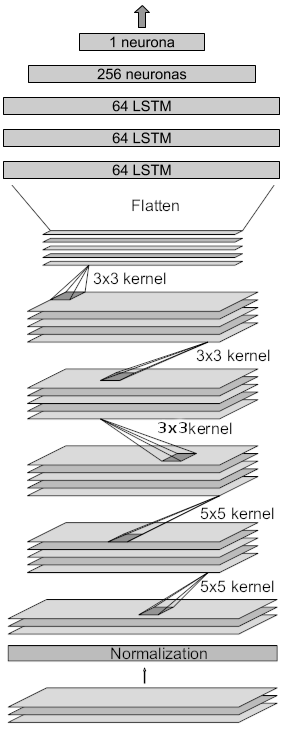
\includegraphics[scale=0.33]{img/chauffeur}}
	\caption{Chauffeur model.}
	\label{fig:chauffeur}
\end{figure}


Similar to \cite{hassan2018convolutional}\cite{pinheiro2014recurrent}, the model depends on distributed time entries. This means that the network requires as input a short succession of chrono-evaluated images. As each image is represented as a 3D tensor, this model requires a 4D tensor related to a scalar, which is the class, in this case the turn command of the last image of the sequence. In Fig. \ref{fig:tensor} the required data structure is shown.

\begin{figure}[h]
	\centerline{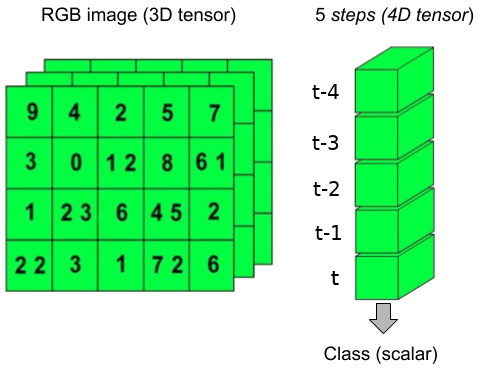
\includegraphics[scale=0.3]{img/tensor}}
	\caption{Data structure required.}
	\label{fig:tensor}
\end{figure}

Therefore, each layer is subdivided into $n$ layers that are governed by the same functions, where $n$ is equivalent to the number of steps. Usually, the output of the last convolutional layer is a matrix, but in this approach the output is represented as a 3D tensor. However, the LSTM layers require a matrix as input, for this a layer of flatten is used. This layer reduces the dimensions of the tensioner as shown in Fig. \ref{fig:flatten}.

\begin{figure}[h]
	\centerline{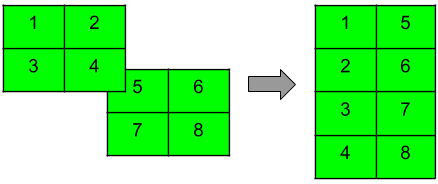
\includegraphics[scale=0.3]{img/flatten}}
	\caption{Transformation made by the flatten layer.}
	\label{fig:flatten}
\end{figure}

\section{Experiments \& results}
In this experiment 2 databases were generated. The first contains a total of $97, 186$ patterns, with a total of $291, 558$ images obtained between the three views. Given that the simulator provides between 9 and 10 patterns per second, there's an approximate total of 2.7 hours of driving on the two tracks. The second database contains only data from the second track, which is longer and more complicated. This database contains $24, 793$ patterns, $74, 379$ images and represents 41 minutes of driving.

To compare the results, we take the model proposed in \cite{bojarski2016end}\cite{bojarski2017explaining} shown in Fig. \ref{fig:pilotnet}. This model called Pilotnet is the largest reference in the self-driving domain and unlike the Chauffeur model (Fig. \ref{fig:chauffeur}), it doesn't have convolutional layers of distributed time and its classification is based only on multilayer perceptron.

\begin{figure}[h]
	\centerline{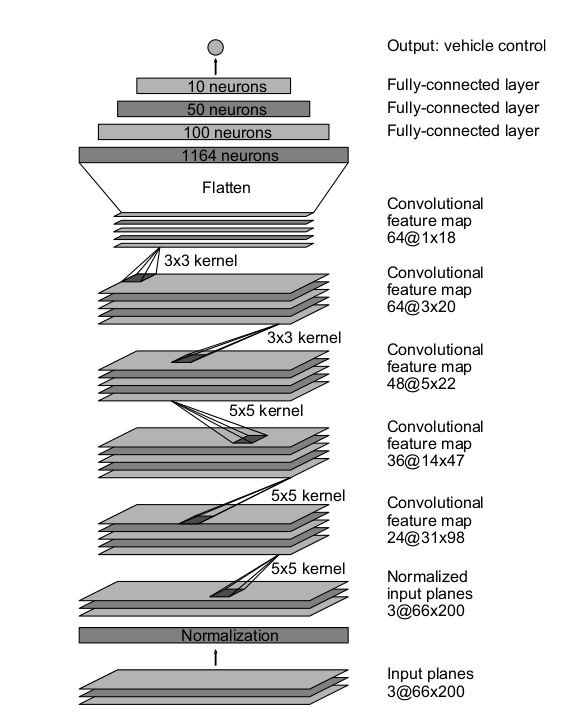
\includegraphics[scale=0.33]{img/pilotnet}}
	\caption{Pilotnet model \cite{bojarski2016end}.}
	\label{fig:pilotnet}
\end{figure}

The tuning of parameters is the same for both models:
\begin{itemize}
	\item Epochs: 10.
	\item Iterations: 10,000.
	\item Lot: 40 patterns.
	\item Learning rate: $1.0^{-5}$.
	\item Training set: 80\%.
	\item Validation set: 20\%.
\end{itemize}

To compare the results with the Chauffeur model with different steps, I trained with 3 and 5 steps using the same parameter configuration.

In the study of the state of the art, few metrics related to the evaluation of autonomy were found. In \cite{bojarski2016end}, the metric shown in \eqref{eq:nvidia} is proposed, which is the most referenced in the literature.

\begin{equation}
autonomy = (1 - \frac{interventions \cdot 6}{elapsed\ time}) \cdot 100
\label{eq:nvidia}
\end{equation}

The metric is based mainly on the corrections made by the driver to avoid collision of the vehicle. This number of interventions is multiplied by a constant of 6 seconds, which represents the average time an average driver takes to correct the course of the vehicle, according to a study carried out by them.

Throughout the tests carried out in this work it was observed thatn't necessarily an intervention is usually 6 seconds in the simulation, even though it's in real time. Due to these variations, the metric proposed in the literature turns out to be less reliable, therefore it's proposed to measure the autonomy based on the intervention time of the driver to correct the address using the expression \ref{eq:proporsed}. This proposed metric evaluates the autonomy similarly to the previous one, with the difference that it takes an absolute time of interventions.

\begin{equation}
autonomy = 100 - \frac{total\ intervention\ time}{elapsed\ time}\cdot 100
\label{eq:proporsed}
\end{equation}

As a third autonomy metric, it's proposed to perform the test without the driver's intervention to measure the percentage of the route that completes the vehicle on the runway until the first collision using the expression \eqref{eq:completed road}. In this way there's a reference on what each model He has learned from the road.

\begin{equation}
completed\ road = \frac{s \cdot t}{d} \cdot 100
\label{eq:completed road}
\end{equation}

Where $s$ is the average speed of the vehicle, $t$ represents the driving time until the first collision or completing the route and $d$ is the total distance of the test track.


First, the test was made allowing the driver's interventions. To activate the manual driving, press the "x" button on the steering wheel, this deactivates the neuronal model commands and initializes the counting of the intervention times. Similarly, by pressing the "$\circ$" button, print the values of the calculated metrics until the moment of the button event. This test was carried out with the two models, the configurations of 3 and 5 steps of the Chauffeur model and with both databases, the results obtained are shown in Table \ref{table:autonomy}.

\begin{table}[H]
	\caption{Metrics of autonomy obtained.}
	\begin{center}
		\begin{tabular}{|c|c|c|c|c|}
			\hline
			\multirow{3}{*}{\textbf{Model}} & \multicolumn{4}{|c|}{\textbf{Metrics}} \\\cline{2-5} 
			& \multicolumn{2}{|c|}{NVIDIA} & \multicolumn{2}{|c|}{Proporsal} \\\cline{2-5} 
			& Road 1 & Road 2 & Road 1 & Road 2 \\\hline \hline
			
			Pilotnet (shortest db) & 44.55\% & 83.11\% & 82.09\% & 96.35\% \\\hline
			Pilotnet (largest db) & \textbf{100\%} & 77.57\% & \textbf{100\%} & 90.05\% \\\hline
			Chauffeur 3 steps (shortest db) & 76.88\% & 85.96\% & 90.26\% & 92.48\% \\\hline
			Chauffeur 3 steps (largest db) & \textbf{100\%} & \textbf{100\%}   & \textbf{100\%} & \textbf{100\%} \\\hline
			Chauffeur 5 steps (shortest db)& 88.89\% & 88.78\% & 95.43\% & 96.23\% \\\hline
			Chauffeur 5 steps  (largest db)& \textbf{100\%} & \textbf{100\%} & \textbf{100\%} & \textbf{100\%} \\\hline
		\end{tabular}
		\label{table:autonomy}
	\end{center}
\end{table}

In a second stage, each model is tested without intervention. When starting the simulation, a chronometer is initialized and it's finalized when the vehicle stops. Every second the speed is sampled to obtain an average speed, this to calculate the percentage of the completed road. The results of this experiment are reported in Table \ref{table:read}.

\begin{table}[H]
	\caption{Metrics of road completed obtained.}
	\begin{center}
		\begin{tabular}{|c|c|c|}
			\hline
			\multirow{2}{*}{\textbf{Model}} & \multicolumn{2}{|c|}{\textbf{Road completed}} \\\cline{2-3} 
			& Road 1 & Road 2 \\\hline \hline
			
			Pilotnet (shortest db) & 9.47\% & 7.52\% \\\hline
			Pilotnet (largest db) & \textbf{100\%} & 30.44\% \\\hline
			Chauffeur 3 steps (shortest db) & 33.61\% & 18.07\% \\\hline
			Chauffeur 3 steps (largest db) & \textbf{100\%} & \textbf{100\%} \\\hline
			Chauffeur 5 steps (shortest db) & 34.37\% & 16.93\% \\\hline
			Chauffeur 5 steps (largest db) & \textbf{100\%} & \textbf{100\%} \\\hline
		\end{tabular}
		\label{table:read}
	\end{center}
\end{table}


Remembering that you have 87 classes, a difference of 0.01 in the prediction represents an absolute error in the metrics that are usually used for the evaluation of neural networks, such as precision, accuracy, etc. However, in the tests, a minimal error doesn't have such a drastic effect on driving, that is why this type of evaluation doesn't turn out to be ideal.

On the other hand, the metrics dedicated to measure the error in the prediction adapt much better to the problem and show better the performance of these networks, since they calculate the difference between the expected and the obtained. A small angle of difference doesn't present as much error, that is why these are the ones that were contemplated to evaluate the training of the networks. The metrics used are: Mean Squared Error \eqref{eq:mse}, Mean Absolute Error \eqref{eq:mae} and Root Mean Squared Error \eqref{eq:rmse}.

\begin{IEEEeqnarray}{lCr}
MSE = \frac{1}{n} \sum_{i=1}^{n} = (\hat{Y_i} - Y_i)^2
\label{eq:mse}\\
MAE = \frac{1}{n} \sum_{i=1}^{n} = |\hat{Y_i} - Y_i|^2
\label{eq:mae}\\
RMSE = \sqrt{\frac{1}{n} \sum_{i=1}^{n} = (\hat{Y_i} - Y_i)^2}
\label{eq:rmse}
\end{IEEEeqnarray}

Performing the analysis of the results obtained, the training with the shortest database obtains better results in the error metrics as seen in Fig. \ref{subfig:2}, \ref{subfig:5} \& \ref{subfig:6}, but in practice and according to the Tables \ref{table:autonomy} \& \ref{table:read}, the training with the base of largest data are the ones that drive the car better. It's also observed that the Accuracy Metric presents very variable results and it doesn't stop to have relation with the rest. Another observation is that the RMSE \eqref{eq:rmse} isn't included in the graph since it gives the same results as the MSE \eqref{eq:mse} in all cases.


\begin{figure}[h]
	\centering
	\begin{subfigure}{0.24\textwidth} 
		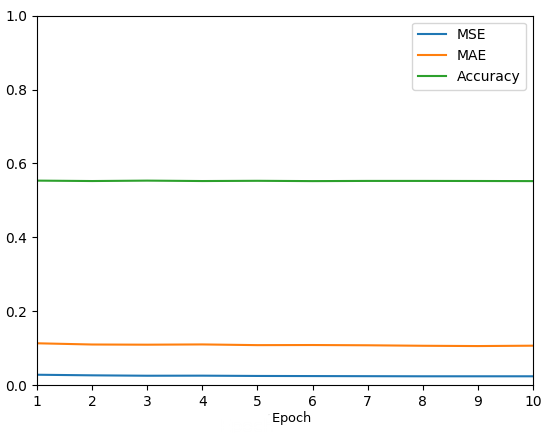
\includegraphics[width=\textwidth]{img/pilotnet1}
		\subcaption{Pilotnet, largest database.} 
		\label{subfig:1}
	\end{subfigure}
	\begin{subfigure}{0.24\textwidth} 
		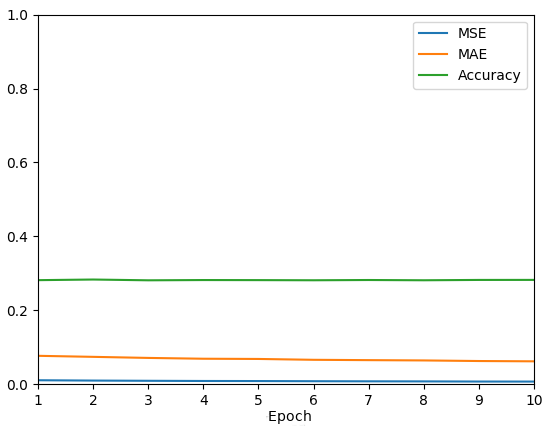
\includegraphics[width=\textwidth]{img/pilotnet2}
		\subcaption{Pilotnet, shorter database.} 
		\label{subfig:2}
	\end{subfigure}
	\begin{subfigure}{0.24\textwidth} 
		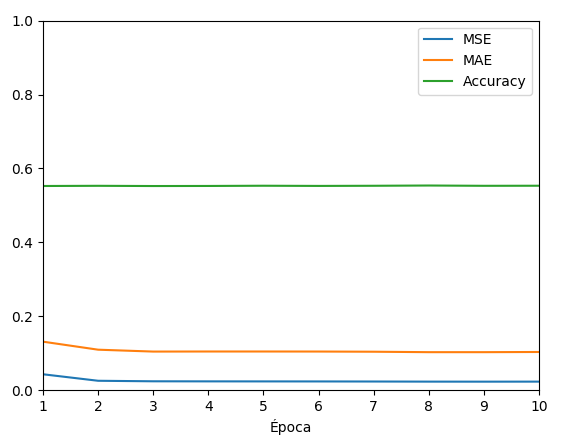
\includegraphics[width=\textwidth]{img/chauffeur3}
		\subcaption{Chauffeur 3 steps, largest database.} 
		\label{subfig:3}
	\end{subfigure}
	\begin{subfigure}{0.24\textwidth} 
		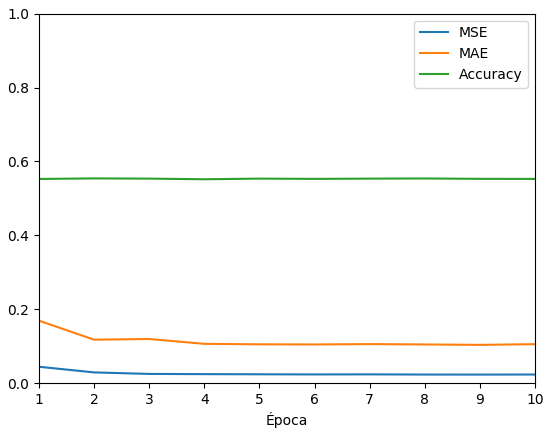
\includegraphics[width=\textwidth]{img/chauffeur5}
		\subcaption{Chauffeur 5 steps, largest database.} 
		\label{subfig:4}
	\end{subfigure}
	\begin{subfigure}{0.24\textwidth} 
		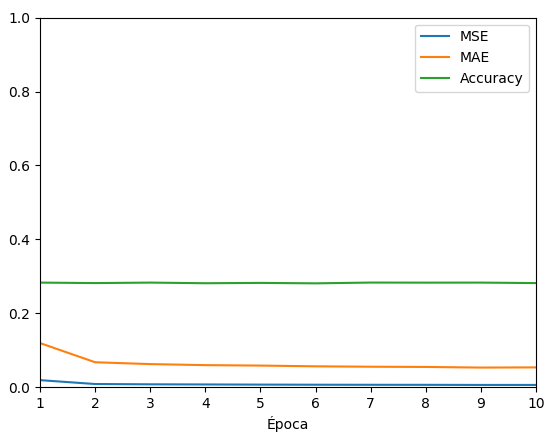
\includegraphics[width=\textwidth]{img/chauffeur3m}
		\subcaption{Chauffeur 3 steps, shorter database.} 
		\label{subfig:5}
	\end{subfigure}
	\begin{subfigure}{0.24\textwidth} 
		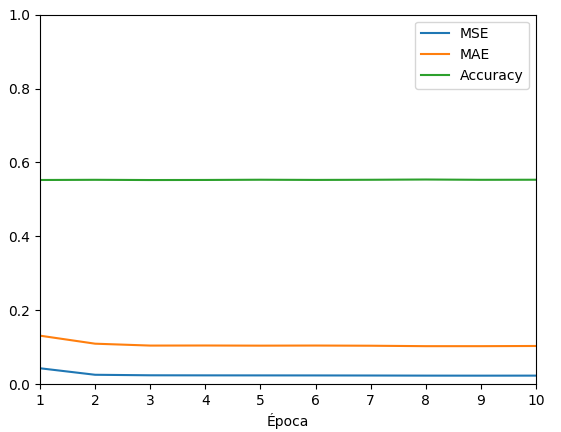
\includegraphics[width=\textwidth]{img/chauffeur5m}
		\subcaption{Chauffeur 5 steps, shorter database.} 
		\label{subfig:6}
	\end{subfigure}
	\caption{Training metrics obtained.} 
	\label{fig:pilottest}
\end{figure}

In the qualitative results, the Chauffeur model shows superiority to the reactive model. Although the experiments done with the 3 and 5 step configurations with the largest database obtain the same results, the driving behavior of the 3-step model is very erratic (as if the driver was in a drunken state). This driving doesn't respect the lanes and although it doesn't collide, it drives near the limits of the road and occasionally moves in zigzag. These behaviors are corrected in the 5-step model, which behaves similarly to a human driver. However, in training with the shortest database it's more sensitive to unknown situations, which doesn't happen with the previous one.


\section{Conclusion}

As a conclusion, a reactive model isn't enough to completely solve a complex problem such as driving. It was shown that a model created to label static images can be adapted to process small video fragments and predict subsequent actions. Although this driving is done in environments without obstacles, it can be used on free roads.

The observation of the erratic behavior of the 3-step model motivated a study of the literature with the intention of finding metrics dedicated to the evaluation of driving behavior. In this study we didn't find any method to evaluate this behavior, so as a future work, the design and experimentation of a metric to evaluate the autonomy as a driving behavior will be carried out. 



\addcontentsline{toc}{section}{Referencias} 
\printbibliography




\end{document}
